\section{Proceso de comisi�n disciplinaria en la Facultad 4}\label{process}
%TODO
%Descripci�n del proceso de comisi�n disciplinaria en la Facultad 4
El proceso de comisi�n disciplinaria comienza cuando un profesor o estudiante de la \uci presenta una denuncia ante el Decano de la Facultad. El Decano de la Facultad es el encargado de verificar la veracidad de la denuncia y de asignar una comisi�n disciplinaria para que investigue el caso. Esta es la encargada de realizar la investigaci�n, lo cual incluye la recopilaci�n de informaci�n hist�rica de cada infractor, declaraciones de implicados y opiniones de los trabajadores que atienden las �reas a las que pertenece cada infractor; y de emitir conclusiones del caso para cada uno. Estas son revisadas por el Decano de la Facultad, el cual, de aceptarlas, emite la resoluci�n del caso y notifica a cada infractor.
\begin{figure}[h]
	\centering
	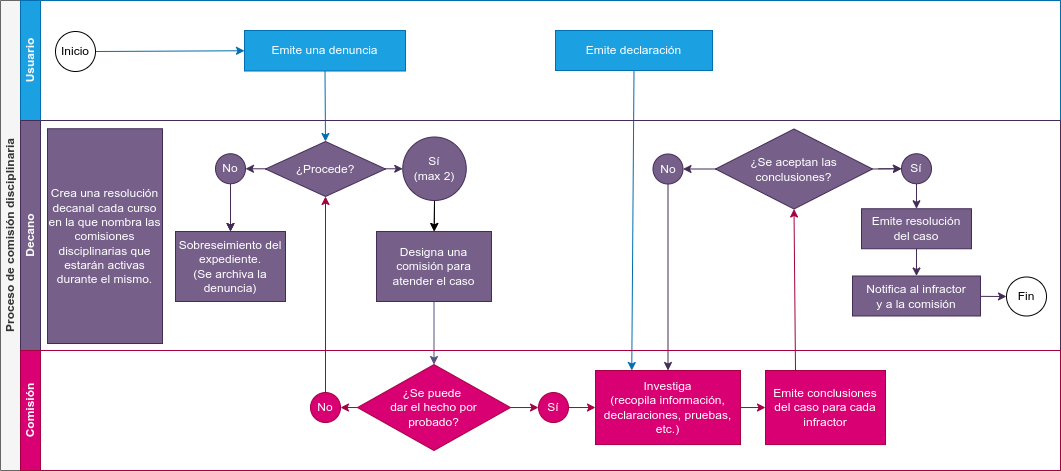
\includegraphics[width=1\textwidth]{images/process.png}
	\caption{Diagrama de actividades que describe el \proceso\ de \lafac}
	\label{fig:activities}
\end{figure}

